\documentclass{article}
\usepackage{graphics}
\begin{document}

\title{Software Requirements Specification for Mashbot} 
\author{George D'Andrea \and \and Andrew Gall \and Josiah Kiehl \and
  Cody Ray \and Vito Salerno}
\date{\today}
\begin{titlepage}
\maketitle
\end{titlepage}

\tableofcontents

\section{Introduction}

\subsection{Purpose} % JK
This document is the general overview of the requirements for the Mashbot 
project.  The sections below are specifically ``what'' is to be done as opposed 
to ``how'' it is to be done.
\subsection{Scope} % JK
This document covers a high level overview of what features a successful project 
delivery will include.
\subsection{Glossary} % Everyone
\subsection{Overview} % CR

\section{Overall Description}
     \subsection{Product Perspective}
		For many startups and small businesses, marketing /
                customer service and business / development efforts
                compete for scarce resources.  Furthermore, early
                stage startups often have small or non-existent
                marketing budgets, especially in resource-hungry
                product-based startups.  Although the plethora of
                widely available and affordable communications
                technology (e.g., social media, VoIP, streaming video,
                etc.) theoretically reduces both capital and operating
                expenditures related to marketing, the quantity of
                such technologies and services effectively creates an
                "opportunity overload" making the process of
                maintaining a focused and effective marketing campaign
                more difficult.  Furthermore, with the number of
                services, technologies, and "specialists" arriving
                each day, its nearly impossible to keep up with all
                the trends much less to fully take advantage of each
                or even monitor them all adequately! As you can see,
                the widespread adoption of communications technology
                is a double-edged sword---there are many more avenues
                for marketing and customer service, but it is much
                more difficult to effectively apply reputation
                management strategies or adequate customer service
                through all channels. This project proposes to build a
                tool to increase the effectiveness and efficiency of
                marketing campaigns and customer service for small to
				medium businesses.
		\subsubsection{System Interfaces} % VS
			Mashbot combines several components to provide the functionality
			required.
			\begin{itemize}
				\item \textbf{Authentication}
				\item \textbf{Campaign Manager Web Interface}
				\item \textbf{Publishing and Aggregation
                                  Platform}
				\item \textbf{Database}
			\end{itemize}
		\subsubsection{User Interface} % JK
                The user interface consists of a web front end
                with tabs to separate the various workflow areas. To
                create content, the user is provided with a calendar
                scheduling tool, and a content editor.  Additionally,
                there is a monitoring dashboard which gives the user a
                view on responses to the content in any given campaign.
                Finally, there is an explore view that gives the user a
                portal with which they can keep tabs on topics of 
                interest in social media.
		\subsubsection{Hardware Interfaces} % VS
                It's a freaking web application.
		\subsubsection{Software Interfaces} % VS
                It's a freaking web application.
		\subsubsection{Communications Interfaces} % VS
                It's a freaking web application.
		\subsubsection{Memory Constraints} % VS
                Server must not crash.
		\subsubsection{Site Adaptation Requirements} % VS
                TODO: Ask Popyack if needed.
	\subsection{Product Functions} % AG
        Mashbot should be able to:
        \begin{enumerate}
          \item Schedule content for various services to be
            published concurrently
          \item View and Compare historical metrics of campaigns
          \item View/Create replies to content
          \item Maintain users and approvers of content
          \item Set up keyword alerts for ``watched'' services
        \end{enumerate}
	\subsection{User Characteristics} % AG
        The target user is a small to medium business employee who understands
        the basic capabilities of social media.
        
	\subsection{Requirements Apportioning} % VS
        \begin{tabular}{|c|p{4in}|}
          \hline
          \textbf{Priority} & \textbf{Description} \\
          \hline \hline
          1 & Mashbot can not be released unless it satisfies these
              requirements. \\
          \hline
          2 & Mashbot may be initially released without satisfying these
              requirements. Having these requirements unfulfilled must
              not create dangers to the system. They should be implemented in the next
              minor release. \\
          \hline
          3 & These requirements are not expected to be fulfilled by
              the initial release of Mashbot, but should be
              implemented in the next major release. \\
          \hline
          4 & These requirements are outside the current scope of the
              project, but are included to exhibit how our software
              will improve in the future. \\
          \hline
        \end{tabular}

\section{Specific Requirements}
	\subsection{External Interface Requirements}
	\subsection{Functional Requirements}
		\subsubsection{User Accounts} % AG
			\begin{itemize}
				\item \textbf{User Account Types and Permissions} The system categorizes users on the basis
				of roles and privileges. Within these roles, the system also categorizes users based on
			 	the roles that they have within individual products.	These are referred to as user 
				account roles.
				\begin{itemize}
					\item Mashbot! Campaigns supports the following account roles:
						\begin{enumerate}
							\item Content Approver
							\item Content Creator
							\item Content Editor
							\item Content Release Scheduler
							\item Content Responder
							\item Group Administrator
							\item System Administrator
						\end{enumerate}
					\item A user may possess more than one role.
					\item Roles reflect actions that can be performed by a user.
					\item Roles can be assigned to a user account for individual products.
					\item \textbf{Content Approver} can approve for release content which has been
					submitted for approval \textbf{Priority 4}
					\item \textbf{Content Creators} may create new content or 
					import existing content into the system. They may also 
					submit this content for approval. \textbf{Priority 4}
					\item \textbf{Content Editor} may edit content which has already been posted to external
					services. \textbf{Priority 4} 
					\item \textbf{Content Release Scheduler} may schedule or 
					immediately initiate the release to external services of 
					content which has already been submitted and 
					approved.\textbf{Priority 4}  
					\item \textbf{Content Responder} may respond to responses 
					which have been made to the posted content within the 
					external services.  \textbf{Priority 4} 
					
					\item \textbf{Worker} have permission to perform any 
					of the subsidiary roles (Content Approver, Content Creator, 
						Content Editor, Content Release Scheduler, and Content 
						Responder) for a particular group.  \textbf{Priority 1}
					
					\item \textbf{Group Administrator} has all the same 
					permissions as a product worker and can create new product
					worker accounts in groups that it owns.\textbf{Priority 1}  
					
					\begin{itemize}
						\item There must be at least one product administrator 
						for each group. \textbf{Priority 1}
					\end{itemize}

					\item \textbf{System Administrator} can perform any of the roles in the system for any product.
					Additionally, they can create Group Administrator 
				accounts.
				\end{itemize}

				\item \textbf{User Account Creation} - New user accounts can be 
				created with the product.
					\begin{itemize}
						\item The system may contain any number of user 
						accounts.
						\item The system allows only anyone to create new 
						Group Administrator accounts.
						\item The system allows only a Group Administrator to 
						create new Worker accounts with membership in 
						its groups.
						\item The system allows anyone to create a new Product 
						Worker account with no group membership.
						\item Certain pieces of information are required to 
						create new account of any kind.
						\item The following information is required for any new 
						user account:
							\begin{itemize}
								\item Username
								\item Password
								\item Name
								\item Email Address
								\item Group Membership
								\item User Account Type
							\end{itemize}	
				
					\end{itemize}
				\item \textbf{User Account Modification} The system allows users 
				to modify their accounts once created. The system also allows 
				Group Administrators to grant existing Workers 
				\begin{itemize}
					\item The system requires that a user have logged in the 
					proper username and password before modifications can be 
					made.
					\item The following user account information is modifiable 
					by all user types:
						\begin{itemize}
							\item Password
							\item Email Address
							\item Name
						\end{itemize}

					\item The following user account information is modifiable
					by all Group Administrators for groups in which they are 
						members and by the System Adminstrator for all groups:
						\begin{itemize}
							\item Group Membership
						\end{itemize}

					\item The following user account information is modifiable
					by the System Administrator only:
						\begin{itemize}
							\item Username
							\item User Account Type
						\end{itemize}
				\end{itemize}
				
				\item \textbf{User Account Deactivation} 
						

			\end{itemize}

		\subsubsection{Marketing Campaigns} % JK
                A campaign is a collection of content that is scheduled to be published by the company using mashbot.
                \begin{itemize}
                  \item Name
                  \item Pieces of content
                  \item Schedule
                  \item User/Group Permissions
                \end{itemize}
                A campaign's schedule is a set of dates and times that a piece of content has some action taken upon in.  Any action can be scheduled: post, edit, delete.
                
				Erexample: A series of tweets, blog posts and you tube videos 
		need to be published for the release of a Product X.  These are all 
		added to a Campaign.  The user may then use the Campaign's calendar to 
		schedule these pieces of content for publishing
		\subsubsection{External Service Accounts} % JK
                An external service account is a set of credentials and/or an authentication token which allows Mashbot to connect to services.  The requirements for ESAs vary from service to service, where one service might provide token based authentication where another will provide only username/password.
	\subsection{Security Requirements} % VS 
	\subsection{Design Constraints} % CR
	\subsection{Software System Attributes} % AG
	\subsection{User Interface} % JK
        The user interface is to be clean and crisp. There is to be a tabbed navigation bar that unifies the sitewide navigation, as well as module specific navigation as needed.
        Tabs:
        \begin{itemize}
        \item Dashboard
        \item Create
        \item Schedule
        \item Explore
        \end{itemize}
        \subsubsection{Dashboard}
        The dashboard consists of graphs and charts to give the user a quick view on how their campaigns are performing.
        Metrics include:
        \begin{itemize}
        \item Clickthrough rate
        \item Page Views
        \item Number of Comments
        \end{itemize}
        Service plugins can define additional specialized metrics to track, as well, for instance ``retweets'' for Twitter.
        A panel is available to give more information on each metric as it is selected.
        \subsubsection{Create}
        This view allows users to create campaigns and fill them with content.  This view is also used when users need to edit an existing campaign.
        \paragraph{Add content}
        A user can add content via the add content button near the top of the view.  This will prompt the user to select the content type, which is populated by the services the user currently has access to via credentials stored in the system. This will create a section in the main part of the view that allows the user to add individual elements of that content type, each individually scheduled.  Each row line item will allow the user to schedule, edit, or delete that content type.
        \subsubsection{Schedule}
        \paragraph{Scheduling content}
        Users can drag items from the left hand bucket of content to the calendar to schedule content.  The content will receive a default golive time of 12am on the day the content is dragged to.  If the user desires a different time, he may click the content in the schedule and assign the proper time.
        \paragraph{Calendar}
        The calendar allows the user to manage when content goes live, and gives a visual representation of the actions taken on content.  It is clear when content goes live and when (if) it is deleted.  The user can page from month to month to schedule content to any day desired.
        \subsubsection{Explore}
        This view allows users to get a pulse on what information social media contains.  This includes the ability to set up monitored searches for services that support keyword search via api.  This also will aggregate data gathered from comments on content that has been published as part of a given campaign
        \paragraph{NICK: What other sort of data mining could we do here?}
        TODO: Mockup for Explore, once we flesh out what this is supposed to be.
        \clearpage
        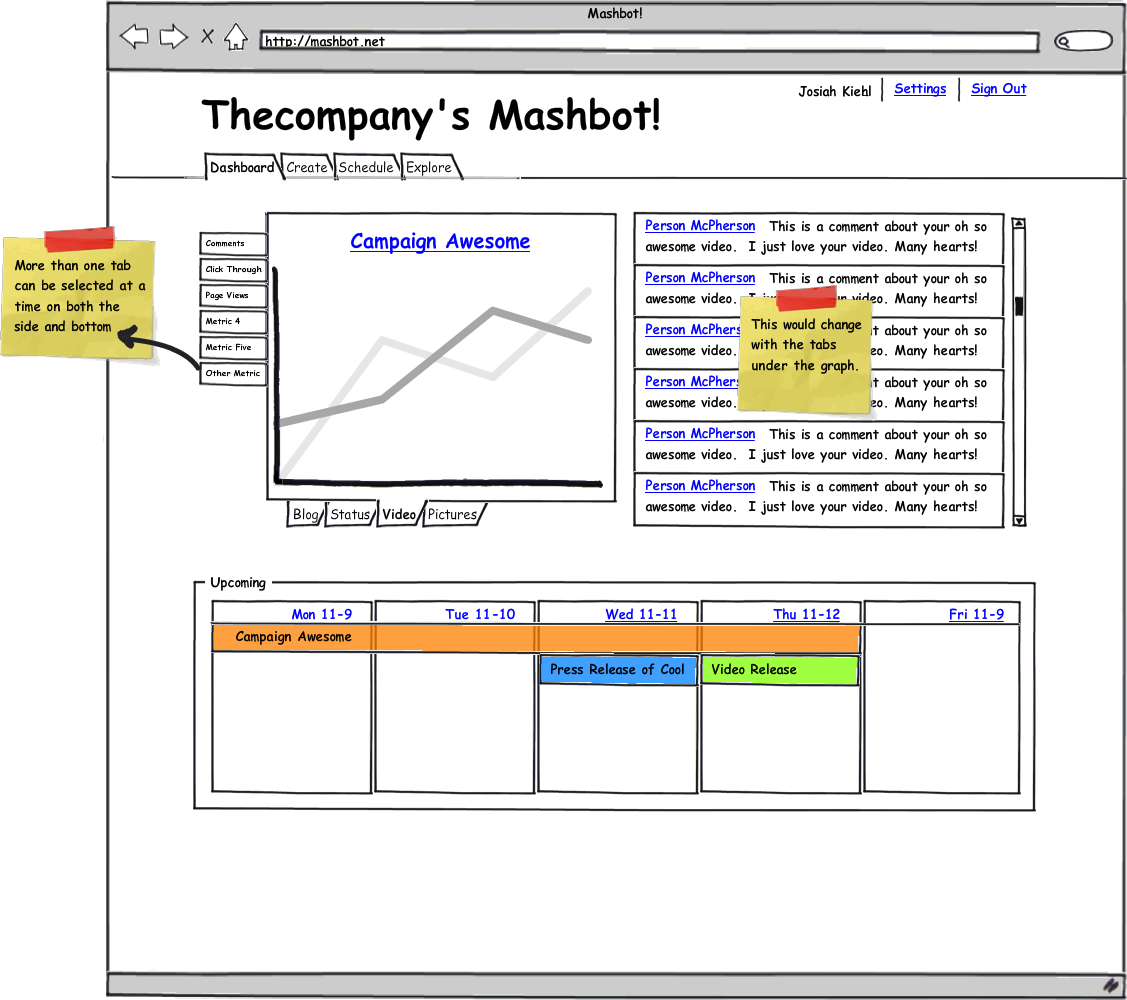
\includegraphics[width=\textwidth]{../mockups/dashboard.png}
        \clearpage
        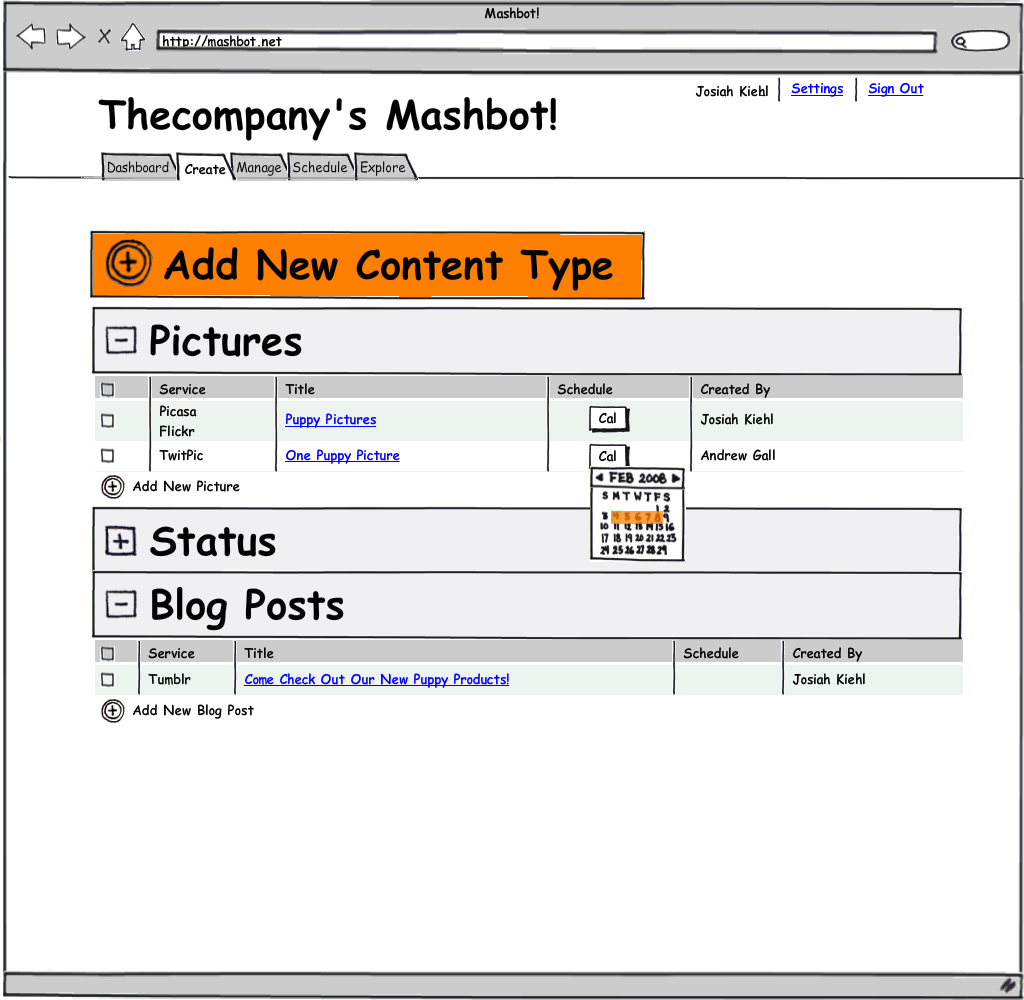
\includegraphics[width=\textwidth]{../mockups/create.png}
        \clearpage
        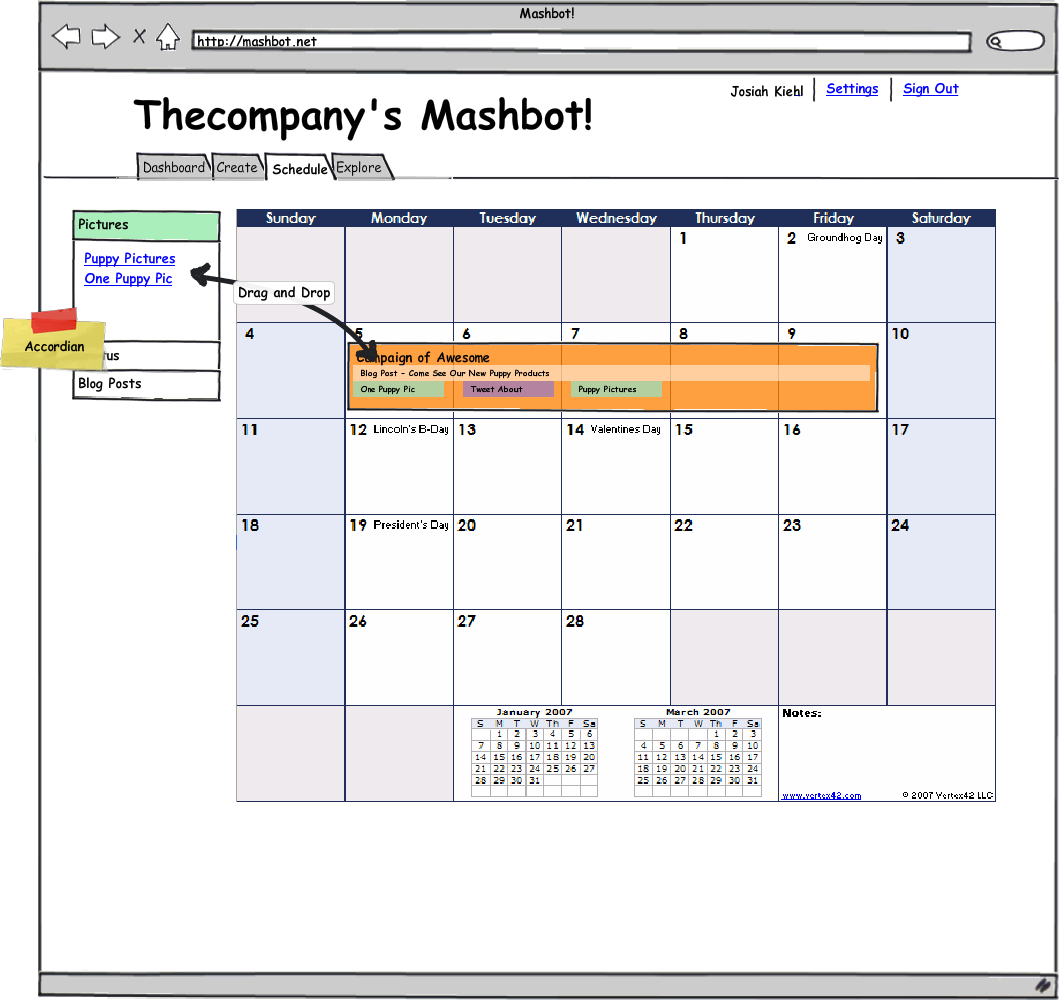
\includegraphics[width=\textwidth]{../mockups/schedule.png}
        \clearpage
\section{Preliminary Analysis} % JK
Mashbot is a data driven web application.  It aggregates data from various web services.  This figure shows the flow of data through the web application.
There is a core that handles all requests for various data needed by the appluication.  Authentication information is retrieved from the database and used to request content from services.
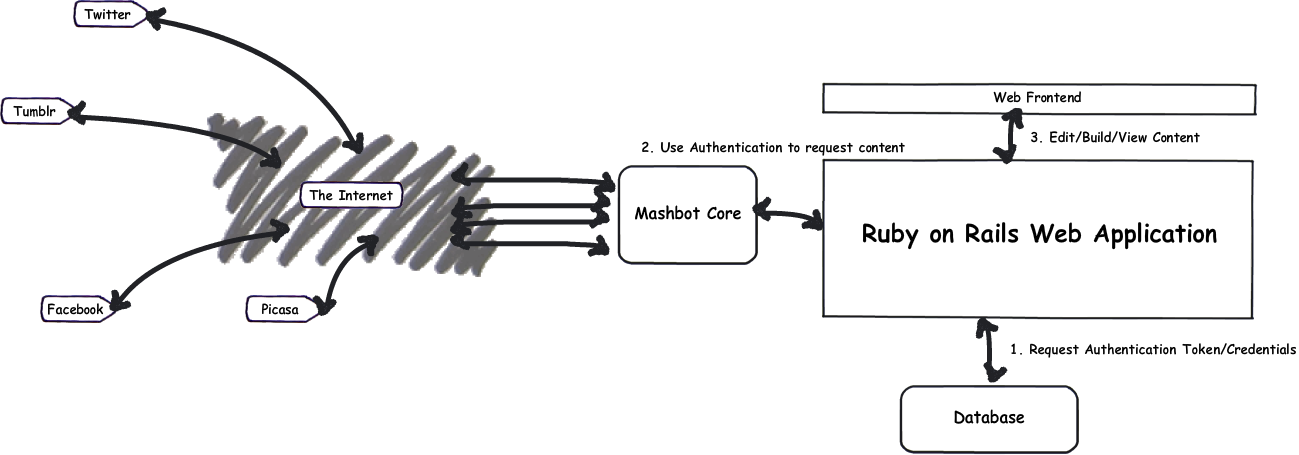
\includegraphics[width=\textwidth]{../mockups/dataflow.png}
\clearpage
\section{Use Cases} % CR

%% \section{IO}

%% Inputs
%%   CRUD
%%   Types
%%     Pictures
%%     Status/Tweet
%%     Blog
%%     Video

%% Users
%%   Name
%%   Email
%%   Company
%%   Permissions
%%   Accounts
    
%% Account
%%   What a company buys
%%   Allows user/campaign creation
  
%% Campaigns
%%   Name
%%   Schedule
%%   Content
%%     Distribution Channels


\end{document}


% LocalWords:  Mashbot
